%use in documents with \subfile{tex/intro}
\documentclass[../../master.tex]{subfiles}

\begin{document}

\subsubsection{Structure Prediction of \textit{Azoarcus}}
\label{ssub:results:azopred}

\paragraph{Minimum Free Energy Predictions.}
\label{par:results:mfepred}

Using the default energy parameter set \texttt{turner2004}, the structure prediction tools introduced in \autoref{sub:methods:sspred} were assessed based on their ability to recover the native structure of the \textit{Azoarcus} group I intron.
For this, the truncated sequence and structure from \autoref{fig:azodata:b} was used.

As summarized in \autoref{tab:predictionstats}, \texttt{RNAfold} had the fastest runtime.
Also, by excluding the positions in P7 from forming base pairs using \texttt{RNAfold}, the base pair distance to the pseudoknot-free target structure was noticeably reduced.
With a value of $\unitfrac[-74.20]{kcal}{mol}$, this prediction yielded the lowest predicted energy in this comparison.
However, adding the computed energy contribution of the missing P7 base pairs from \autoref{fig:p7energy:a}, an adjusted value of $\unitfrac[-77.10]{kcal}{mol}$ is somewhat more in line with the other MFE predictions. %\todo{this is without dangling ends, though; it is still similar to the unconstrained prediction}.

\begin{table}[!ht]
	\centering\setstretch{0.95}
	\caption[Runtime and Accuracy of Different Prediction Methods]{The different tools were tested on the \textit{Azoarcus} Group I intron (see \autoref{fig:azodata:b}). 
		$\Delta G$: Gibb's free energy of the predicted structure, $\operatorname{d}_{\mathrm{bp}}$: base pair distance to the assumed native structure (with pseudoknots except values marked with $*$). Here, the default \texttt{turner2004} parameters were used.
		See \autoref{tab:mfepredazo} for the concrete predicted structures.
	}
	\label{tab:predictionstats}
	\begin{tabularx}{1\textwidth}{lrrrX} \toprule
		\textbf{Tool} & Runtime & $\Delta G$ & $\operatorname{d}_{\mathrm{bp}}$ & Notes \\ \midrule
		\texttt{RNAfold} & \unit[55]{ms} &  \unitfrac[-77.40]{kcal}{mol} & $45^*$ & --- \\
		\texttt{RNAfold} & \unit[49]{ms} &  \unitfrac[-74.20]{kcal}{mol} & $29^*$ & base pairs at P7 were forbidden \\ \midrule
		\texttt{RNAPKplex} & \unit[191]{ms} & \unitfrac[-77.40]{kcal}{mol} & $51\hphantom{^*}$ & default pseudoknot penalty \\
		\texttt{RNAPKplex} & \unit[595]{ms} & \unitfrac[-79.80]{kcal}{mol} & $53\hphantom{^*}$ & no pseudoknot penalty \\ \midrule
		\texttt{pKiss} & \unit[683]{ms} & \unitfrac[-83.90]{kcal}{mol} & $56\hphantom{^*}$ & default H-type penalty \\
		\texttt{pKiss} & \unit[674]{ms} & \unitfrac[-81.60]{kcal}{mol} & $32\hphantom{^*}$ & H-type penalty $= \unitfrac[9.8]{kcal}{mol}$ \\
		\bottomrule
	\end{tabularx}
\end{table}

Dot plots of the unconstrained and constrained \texttt{RNAfold} prediction confirm that applying this type of constraint improves the prediction of the rest of the structure, although some new false interactions appear (Figure \ref{fig:rnafold_constraint}).

\begin{figure}[!ht]
	\centering
	\begin{subfigure}[t]{0.5\textwidth}
		\centering
		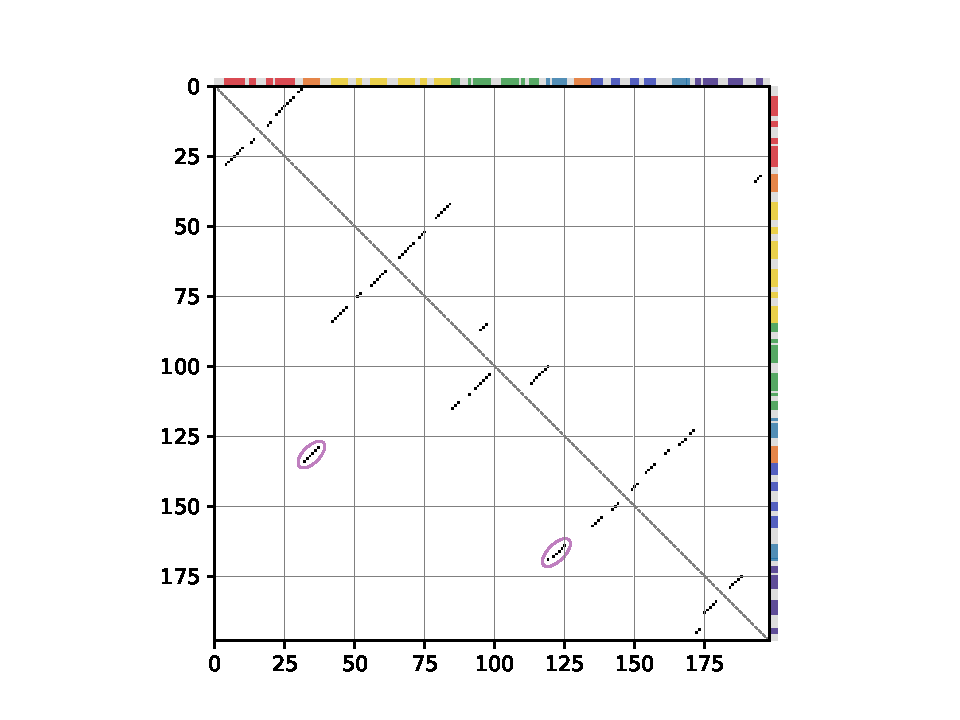
\includegraphics[trim=55 10 70 10, clip, width=\textwidth]{pic/results/designs/dotplots/azo_rnafoldpred.pdf}
		\caption{no constraints were applied during prediction.
		}\label{fig:rnafold_constraint:a}
	\end{subfigure}%
	\begin{subfigure}[t]{0.5\textwidth}
		\centering
		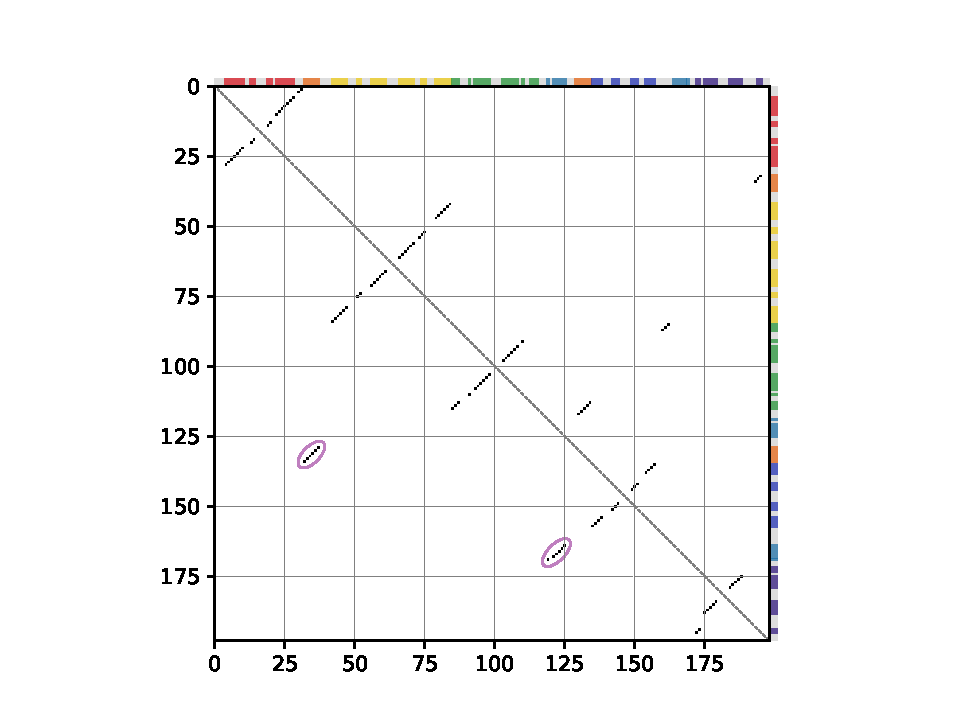
\includegraphics[trim=55 10 70 10, clip, width=\textwidth]{pic/results/designs/dotplots/azo_rnafoldpred_p7constraint.pdf}
		\caption{positions in P7 were excluded from forming base pairs.
		}\label{fig:rnafold_constraint:b}
	\end{subfigure}
	\caption[Constraining \texttt{RNAfold} Prediction]{
		The structure of the \textit{Azoarcus} Group I intron as predicted by \texttt{RNAfold} with 
		\begin{enumerate*}[label={(\alph*)}, font={\bfseries}]
			\item no structural constraints and
			\item structural constraints at P7 positions disallowing base pairs.
		\end{enumerate*}
		The lower diagonal half of these figures shows the target structure, the upper diagonal half contains the prediction.
		Base pairs between two positions are indicated as black squares with position indices labelled at both axes.
		Helices of the native structure are color-coded on top and at the right according to \autoref{fig:azostructure}.
		The location of the original P3-P7 pseudoknot is highlighted in purple.
	}\label{fig:rnafold_constraint}
\end{figure}

Changing the pseudoknot penalty of \texttt{RNAPKplex} did not produce dramatic changes in its structure prediction (\autoref{tab:predictionstats}).
However, for the rest of this work, the pseudoknot penalty of \texttt{RNAPKplex} was set to zero to be approximately consistent with the constrained \texttt{RNAfold} prediction.
%\newpage
Increasing the H-type initiation penalty of \texttt{pKiss} to $\unitfrac[9.8]{kcal}{mol}$ notably improved the base pair distance of the prediction to the target structure (\autoref{tab:predictionstats}).
In fact, the MFE structure predicted using the increased penalty recovered the pseudoknot formed by P3 and P7 almost completely (Figure \ref{fig:pkiss_hpenalty}), which is why this modified penalty was used with \texttt{pKiss} throughout this work.

\begin{figure}[!ht]
	\centering
	\begin{subfigure}[t]{0.5\textwidth}
		\centering
		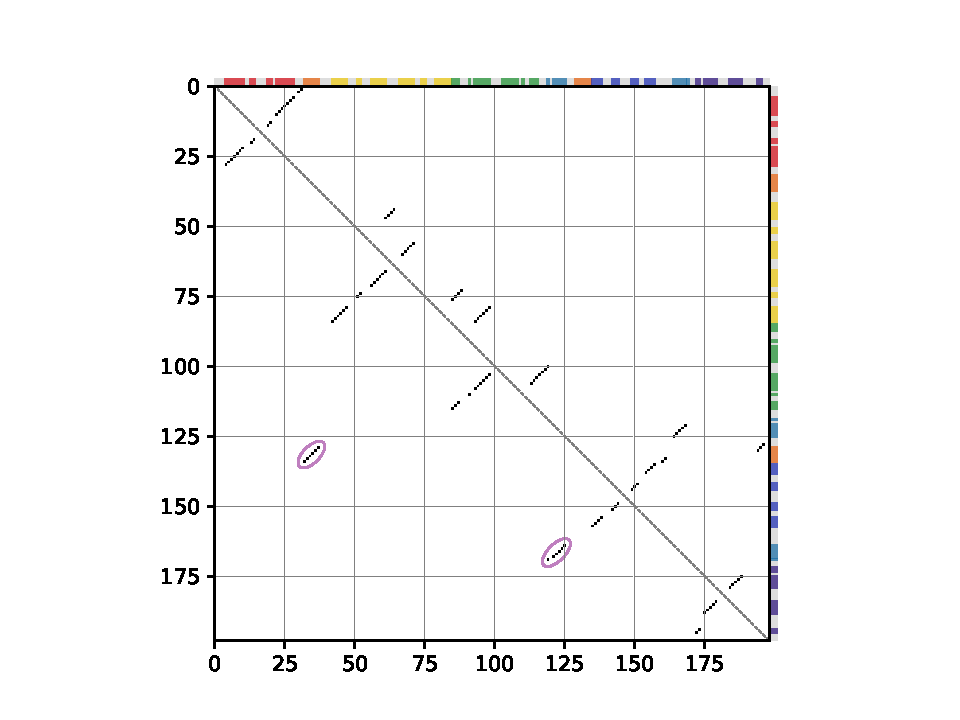
\includegraphics[trim=55 10 70 10, clip, width=\textwidth]{pic/results/designs/dotplots/azo_pkisspred_90.pdf}
		\caption{\texttt{--Hpenalty 9.0}
		}\label{fig:pkiss_hpenalty:a}
	\end{subfigure}%
	\begin{subfigure}[t]{0.5\textwidth}
		\centering
		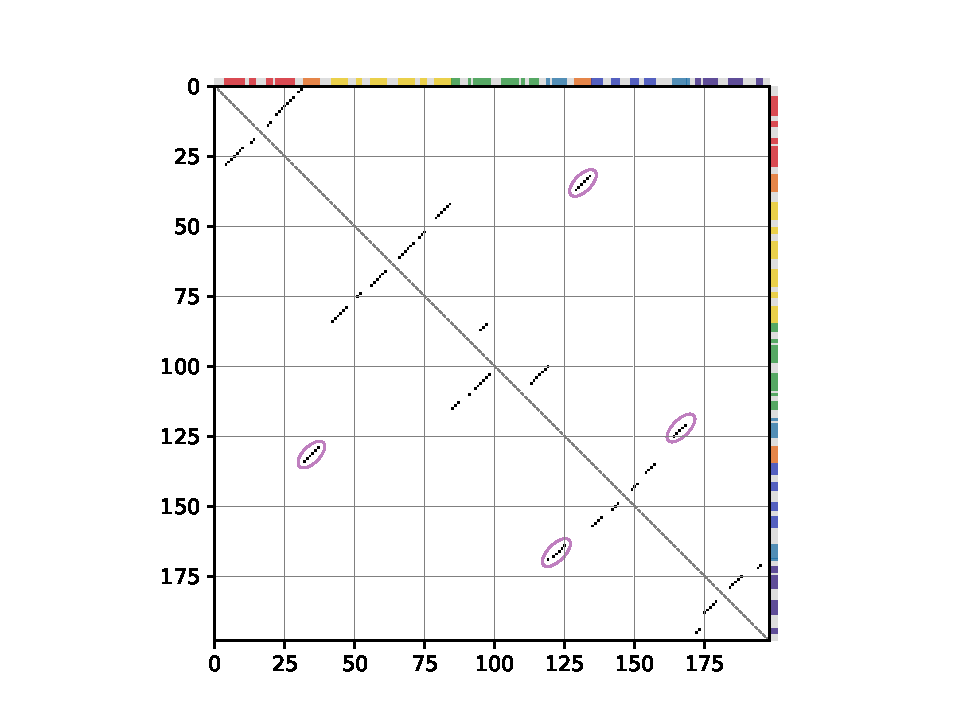
\includegraphics[trim=55 10 70 10, clip, width=\textwidth]{pic/results/designs/dotplots/azo_pkisspred_98.pdf}
		\caption{\texttt{--Hpenalty 9.8}
		}\label{fig:pkiss_hpenalty:b}
	\end{subfigure}
	\caption[Influence of the H-Type Pseudoknot Penalty on \texttt{pKiss}]{
		The structure of the \textit{Azoarcus} Group I intron as predicted by \texttt{pKiss} with different penalties for H-type pseudoknots:
		\begin{enumerate*}[label={(\alph*)}, font={\bfseries}]
			\item the default penalty of \unitfrac[9.0]{kcal}{mol} does not recover the pseudoknot formed between P3 and P7.
			\item a modified penalty of \unitfrac[9.8]{kcal}{mol} recovers the pseudoknot of the target almost completely. Note the mispredicted structure of P6 in the center of the dot plot.
		\end{enumerate*}
		The lower diagonal half of these figures shows the target structure, sthe upper diagonal half contains the prediction.
		Base pairs between two positions are indicated as black squares with position indices labelled at both axes.
		Helices of the native structure are color-coded on top and at the right according to \autoref{fig:azostructure}.
		The location of the original P3-P7 pseudoknot is highlighted in purple.
	}\label{fig:pkiss_hpenalty}
\end{figure}

Only a single base pair of the pseudoknot was missing in the predicted structure due to limitations of the heuristic model of the algorithm not including pseudoknots with bulges \parencite{reeder_design_2004} (\autoref{fig:pkiss_hpenalty:b}).
The most prominent inaccuracy of the prediction in \autoref{fig:pkiss_hpenalty:b} corresponds to the P6 region of the native structure.
However, P6 is part of the scaffold domain of the \textit{Azoarcus} ribozyme and not directly required for catalytic activity.
For this reason, the misprediction of this region was assumed negligible.

More general heuristics implemented in \texttt{pKiss} have the same limitation of not modelling bulges in pseudoknots and were disregarded for this reason and due to their time and memory complexity.
Although this limitation also means that \texttt{pKiss} cannot calculate the free energy of the target structure given the native sequence, this is a relatively minor problem.

By removing the bulge position of P7 as displayed in \autoref{fig:p7energy:b}, the free energy of the modified target structure can be calculated using \texttt{pKiss} and yields
a value of $\Delta G = \unitfrac[-80.90]{kcal}{mol}$.
Adjusting this result by the difference of including the bulge via the values in Figure \ref{fig:p7energy},
the native structure has a free energy of approximately $\Delta G = \unitfrac[-77.10]{kcal}{mol}$ (or $\Delta G = \unitfrac[-76.30]{kcal}{mol}$ with the modified H-type pseudoknot penalty).

\begin{figure}[!ht]
	\centering
	\begin{subfigure}[t]{0.5\textwidth}
		\centering
		\begin{minipage}[b][3cm][c]{0.5\textwidth}
			\large
			\begin{verbatim}
				AGAGACUAG&AUAGUCCA
				.(.(((((.&.)))))).
			\end{verbatim}
			\begin{equation*}
				\Delta G = \unitfrac[-2.90]{kcal}{mol}
			\end{equation*}
		\end{minipage}
		\caption{Base pairs of P7 with a \unit[1]{nt} bulge in dot-bracket notation and the free energy relative to the open chain.
		}\label{fig:p7energy:a}
	\end{subfigure}%
	\begin{subfigure}[t]{0.5\textwidth}
		\centering
		\begin{minipage}[b][3cm][c]{0.5\textwidth}
			\large
			\begin{verbatim}
				AGGACUAG&AUAGUCCA
				.((((((.&.)))))).
			\end{verbatim}
			\begin{equation*}
				\Delta G = \unitfrac[-6.70]{kcal}{mol}
			\end{equation*}
		\end{minipage}
		\caption{Removing the bulged position from P7 stabilizes the stack.
		}\label{fig:p7energy:b}
	\end{subfigure}%
	\caption[Free Energy of the P7 Helix]{Free energy of the base pairs in the region P7 of the \textit{Azoarcus} group I intron
		\begin{enumerate*}[label={(\alph*)}, font={\bfseries}]
			\item with the \unit[1]{nt} bulge present and
			\item without the \unit[1]{nt} bulge present.
		\end{enumerate*}
		Computed with \texttt{RNAeval -d 0} and the default energy parameters.
	}\label{fig:p7energy}
\end{figure}


\paragraph{Partition Function Predictions.}
\label{par:results:partfuncpred}

Following the observation of potential pseudoknots using partition function algorithms (see \autoref{sub:theory:pseudoknots}), base pair probability matrices of the \textit{Azoarcus} group I intron were computed via the McCaskill algorithm implementation of \texttt{ViennaRNA} and the partition function algorithm of \texttt{NUPACK} (Figure \ref{fig:bpp_gissd}).

\begin{figure}[!ht]
	\centering
	\begin{subfigure}[t]{0.5\textwidth}
		\centering
		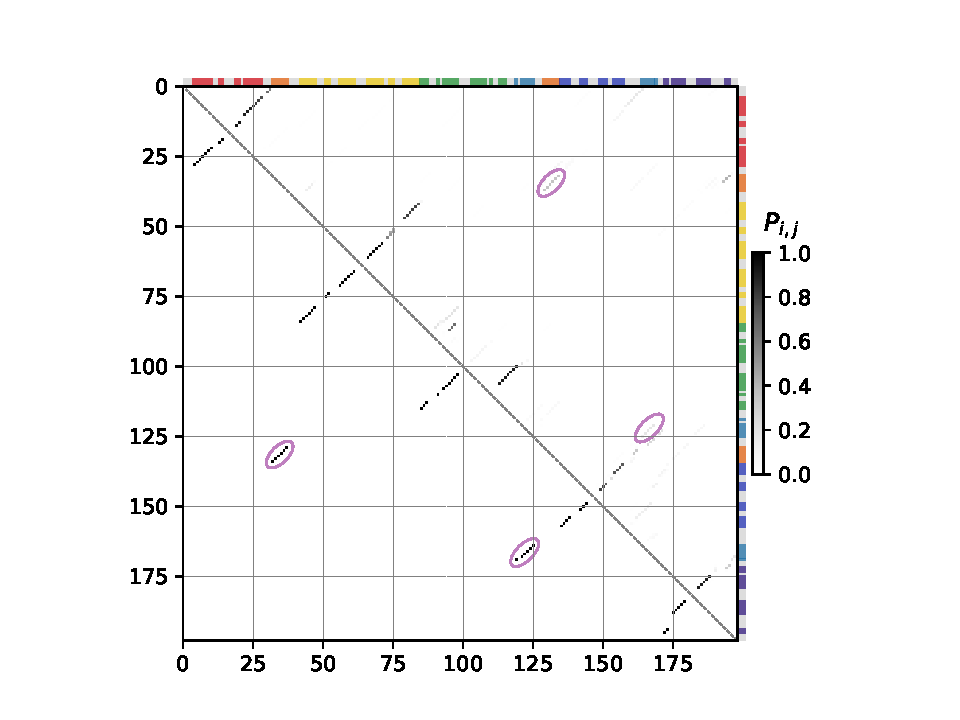
\includegraphics[trim=50 10 70 10, clip, width=\textwidth]{pic/results/designs/dotplots/dot_azo_gissd_viennarna.pdf}
		\caption{Base pair probabilities of the sequence as computed by the implementation of the McCaskill algorithm implemented in \texttt{ViennaRNA}. %\parencite{mccaskill_equilibrium_1990, lorenz_viennarna_2011}.
		}\label{fig:bpp_gissd:a}
	\end{subfigure}%
	\begin{subfigure}[t]{0.5\textwidth}
		\centering
		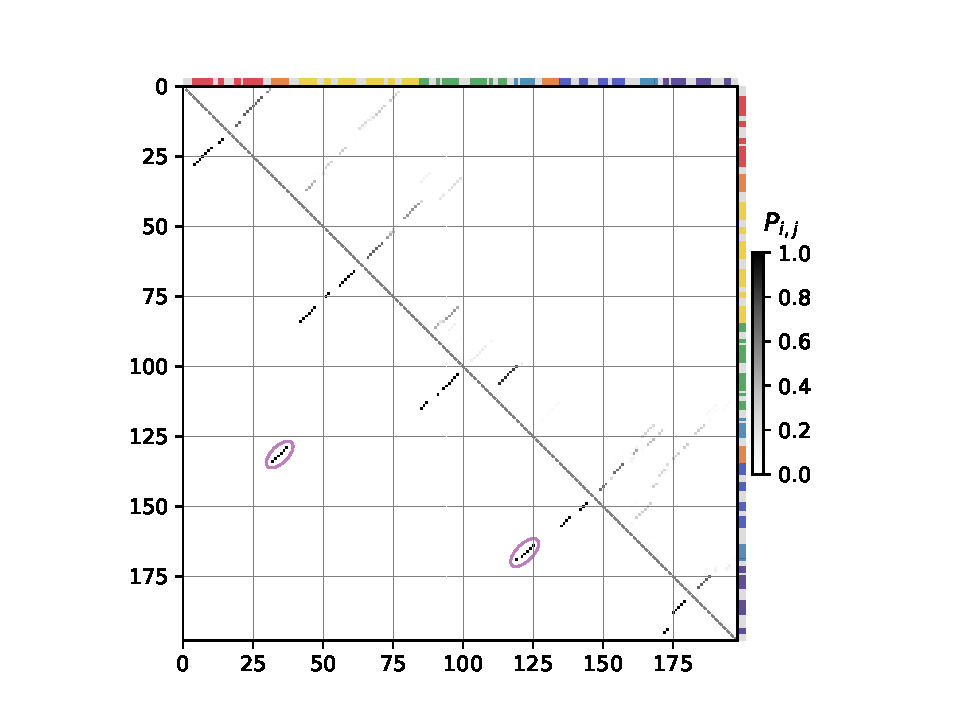
\includegraphics[trim=50 10 70 10, clip, width=\textwidth]{pic/results/designs/dotplots/dot_azo_gissd_nupack.pdf}
		\caption{Base pair probabilities of the sequence as computed by the partition function algorithm implemented in \texttt{NUPACK}. %\parencite{zadeh_nupack_2011, dirks_partition_2003}.
		}\label{fig:bpp_gissd:b}
	\end{subfigure}
	\caption[Base Pair Probabilities of the \texttt{GISSD} Sequence]{
		Dot plots displaying base pair probabilities for the \textit{Azoarcus} group I intron computed by
		\begin{enumerate*}[label={(\alph*)}, font={\bfseries}]
			\item a partition function not explicitly modelling pseudoknots
			\item a partition function accounting for pseudoknotted structures in the ensemble.
		\end{enumerate*}
		The lower diagonal half of these figures shows the target structure.
		Position indices of $P_{i,j}$ are labelled at both axes.
		Helices of the native structure are color-coded on top and at the right according to \autoref{fig:azostructure}.
		The location of the original P3-P7 pseudoknot is highlighted in purple. 
	}\label{fig:bpp_gissd}
\end{figure}

Indeed, non-zero probabilities were predicted for positions close to the pseudoknot present in the native structure, despite using a partition function of a Boltzmann ensemble of nested structures (\autoref{fig:bpp_gissd:a}).

The base pair probabilities predicted by \texttt{NUPACK} did not match the native pseudoknot despite modelling pseudoknots in their algorithm. (\autoref{fig:bpp_gissd:b}).


\paragraph{Energy Parameter Sets.}
\label{par:results:eparams}

So far, only the default energy parameters \texttt{turner2004} have been used to examine the minimum free energy structure prediction quality of the tools used for this specific ribozyme.

In Figure \ref{fig:eparams}, both free energy and base pair distance to the target structure are shown for multiple sets of energy parameters that were introduced in \autoref{tab:eparamsets}.
Most of the parameter sets used here were generated using computational methods.
Only \texttt{turner1999} and \texttt{turner2004} contain parameters obtained from experimental measurements.

Although some of the computationally generated parameter sets showed promising improvements on \texttt{turner2004}, the decisions made here were conservative to prevent overfitting in the design pipeline.

\begin{figure}[!ht]
	\centering
	\begin{subfigure}[t]{\textwidth}
		\centering
		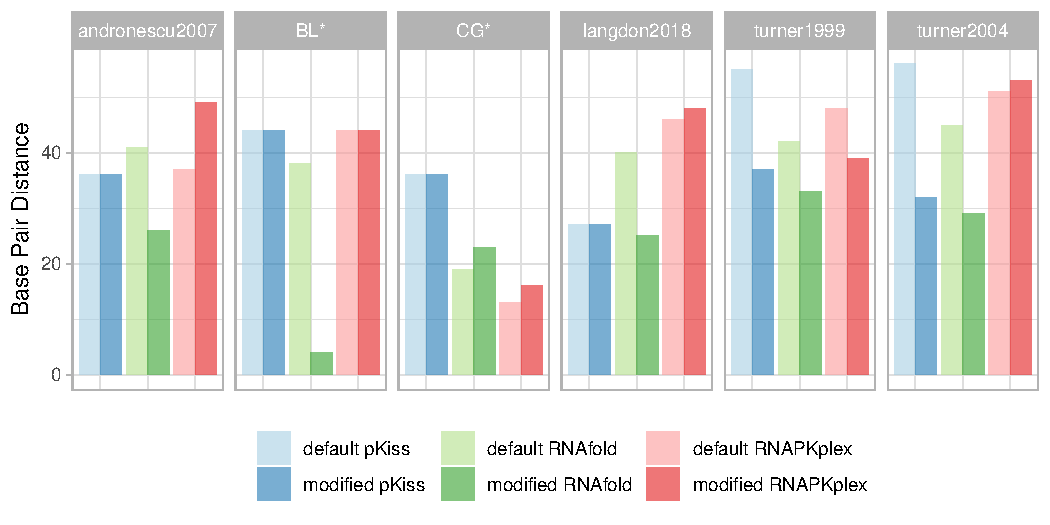
\includegraphics[trim=0 60 0 0, clip, width=0.9\textwidth]{pic/results/eparams/eparams_bpdistance.pdf}
		\caption{
		}\label{fig:eparams:a}
	\end{subfigure}%
	\\
	\begin{subfigure}[t]{\textwidth}
		\centering
		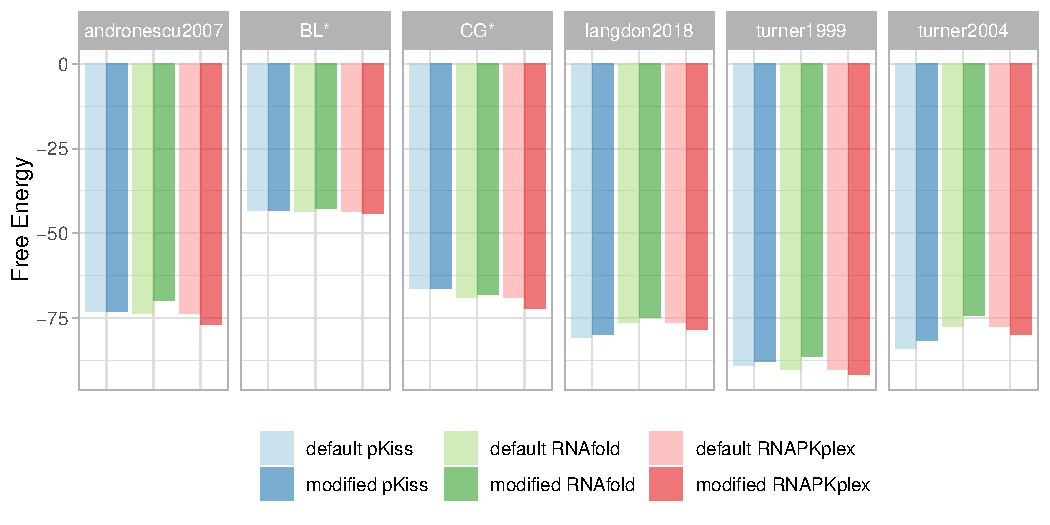
\includegraphics[trim=0 10 0 0, clip,width=0.9\textwidth]{pic/results/eparams/eparams_freeenergy.pdf}
		\caption{
		}\label{fig:eparams:b}
	\end{subfigure}
	\caption[\textit{Azoarcus} Structure Prediction With Different Energy Parameter Sets]{
		Minimum free structure predictions of the \textit{Azoarcus} group I intron using the same tools and modifications as in \autoref{tab:predictionstats} but with different energy parameter sets (see \autoref{tab:eparamsets}):
		\begin{enumerate*}[label={(\alph*)}, font={\bfseries}]
			\item the predicted base pair distance to the target structure and
			\item the free energy of the predicted structure.
		\end{enumerate*}
		Note that the values for \texttt{turner2004} in the rightmost column correspond to \autoref{tab:predictionstats}.
	}\label{fig:eparams} 
\end{figure}

As seen in \autoref{fig:eparams:a}, \texttt{BL*} greatly improved the base pair distance of the constrained \texttt{RNAfold} prediction (green) compared to every other parameter set.
However, due to the substantial deviation of the predicted free energy from every other parameter set used (\autoref{fig:eparams:b}), the biological irrelevance of the prediction using these parameters was a significant concern.

Both \texttt{CG*} and \texttt{andronescu2007} were ruled out because the pseudoknot formed by P3 and P7 was not recovered at all by \texttt{pKiss} with these parameters (not shown, cf. \autoref{sub:appendix:code_availability}). 
Although the base pair distance of the \texttt{RNAPKplex} prediction improved noticeably using \texttt{CG*}, the pseudoknot was not recovered as well.

Generally, predictions made with \texttt{RNAPKplex} were somewhat imprecise. 
Still, \texttt{RNAPKplex} predicted suboptimal structures with pseudoknots similar to the native structure, and was only used in conjunction with \texttt{RNAfold} and \texttt{pKiss} to assess quality of designed sequences (\autoref{ssub:methods:selection}).
Only \texttt{langdon2018} yielded potentially useful improvements; both \texttt{pKiss} variants recovered the pseudoknot as well as with \texttt{turner2004} and the modified pseudoknot penalty.
Still, the improvement relative to the default parameter set consisted of only a few base pairs for the already adjusted methods (constrained \texttt{RNAfold} and \texttt{pKiss} with a penalty of $\unitfrac[9.8]{kcal}{mol}$).

Since the goal was to use designed sequences in experiments eventually, the conservative choice of the default parameter set \texttt{turner2004} seemed reasonable and justified.

\end{document}
